\documentclass{article}
\newtheorem{thm}{Theorem}
\setlength{\oddsidemargin}{0.25in}
\setlength{\textwidth}{6in}
\setlength{\topmargin}{-0.25in}
\setlength{\headheight}{0.3in}
\setlength{\headsep}{0.2in}
\setlength{\textheight}{9in}
\setlength{\footskip}{0.1in}
\usepackage{multirow}
\usepackage{fullpage}
\usepackage{graphicx}
\usepackage{amsthm}
\usepackage{amssymb}
\usepackage{url}
\usepackage{amsfonts}
\usepackage{algpseudocode}
\usepackage{mathtools}

\newcommand{\quotes}[1]{``#1''}

\usepackage{hyperref}
\hypersetup{
    colorlinks=true,
    linkcolor=blue,
    filecolor=magenta,      
    urlcolor=blue,
}


\usepackage{listings}
\usepackage{xcolor} 
 
\lstset{numbers=left, 
        numberstyle=\tiny, 
        keywordstyle=\color{blue}, 
        commentstyle=\color[cmyk]{1,0,1,0}, 
        frame=single, 
        breaklines, 
        extendedchars=false, 
        xleftmargin=2em,xrightmargin=2em, aboveskip=1em, 
        tabsize=4, 
        showspaces=false 
       }

\begin{document}

\title{Homework 3\\ Introduction to Data Analysis and Mining \\ Spring 2018\\ CSCI-B 365}         % Enter your title between curly braces
\author{Instructor: Hasan Kurban\\ Siyi Xian}        % Enter your name between curly braces
\date{February 25, 2018}          % Enter your date or \today between curly braces
\maketitle
All the work herein is solely mine.
\makeatother     % `@' is restored as a "non-letter" character
\pagestyle{plain}
\section*{Directions}
Please follow the syllabus guidelines in turning in your homework.  I am providing the \LaTeX{} of this document too. This homework is due Monday, Feb  26, 2018 10:00p.m. \textbf{OBSERVE THE  TIME}. Absolutely no homework will be accepted after that time. All the work should be your own.  Within a week, AIs can contact students to examine code; students must meet within three days.  The session will last no longer than 5 minutes.  If the code does not work, the grade for the program may be reduced.  Lastly, source code cannot be
 modified post due date.
 
 
 
\section*{ $k$-means Algorithm in Theory}
This part is provided to help you implement $k$-means clustering algorithm.

{\small
\begin{center}
\begin{algorithmic}[1]\label{kmeans}
\State{\bf ALGORITHM} \texttt{k-means}
\State {\bf INPUT} (\textsf{data} $\Delta$, distance $d:\Delta^2\rightarrow \mathbb{R}_{\geq 0}$, \textsf{centoid number} $k$, \textsf{threshold} $\tau$)
\State {\bf OUTPUT} (\textsf{Set of centoids} $\{c_1, c_2, \ldots, c_k\}$)
\State
\State \texttt{***} $Dom(\Delta)$ denotes domain of data.
\State
\State \texttt{***} Assume centroid is structure $c = (v \in DOM(\Delta), B\subseteq \Delta)$
\State  \texttt{***} $c.v$ is the centroid value and $c.B$ is the set of nearest points.
\State \texttt{***}  $c^{i}$ means centroid at $i^{th}$ iteration. 
\State
\State $i = 0$
\State \texttt{***} Initialize Centroids
\For{$j = 1,k$}
\State $c_j^i.v \gets  random(Dom(\Delta))$
\State $c_j^i.B \gets \emptyset$
\EndFor
\State
\Repeat
\State $i \gets i + 1$
\State \texttt{***} Assign data point to {\it nearest} centroid
\For {$\delta \in \Delta$}
\State $c_j^i.B \gets c.B \cup \{\delta\}$, where $\min_{c_j^i}\{d(\delta, c_j^i.v)\}$
\EndFor
\For {$j = 1, k$}
\State \texttt{***} Get size of centroid
\State $n \gets |c_j^i.B|$
\State \texttt{***} Update centroid with average 
\State $c_j^i.v \gets (1/n)\sum_{\delta \in c_j^i.B} \delta$
\State \texttt{***} Remove data from centroid
\State $c_j^i.B \gets \emptyset$
\EndFor
\State \texttt{***} Calculate scalar product (abuse notation and structure slightly)
\State \texttt{***} See notes
\Until{$((1/k)\sum_{j=1}^k~|| c^{i-1}_j-c^{i}_j||) < \tau$}
\State {\bf return} ($\{c_1^i, c_2^i, \ldots, c_k^i\}$) 
\end{algorithmic}
\end{center}}
\subsection*{$k$-means on a tiny data set.}
Here are the inputs:
\begin{eqnarray}
\Delta &=& \{  (2, 5),  (1,5) , (22, 55), (42, 12), (15,16)\}\\
d((x_1, y_1) ,(x_2, y_2)) &=& [(x_1-x_2)^2 + (y_1 - y_2)^2)]^{1/2}\\
k &=&2\\
\tau &=& 10
\end{eqnarray}

Observe that $Dom(\Delta) = \mathbb{R}^2$.  We now work through $k$-means. We ignore the uninformative assignments.  We remind the reader that $\mathsf{T}$ means transpose.

\begin{center}
\begin{algorithmic}[1]
\State $i \gets 0$
\State \texttt{***} Randomly assign value to first centroid.
\State $c^0_1.v \gets random(Dom(\Delta)) = (16,19)$
\State \texttt{***} Randomly assign value to second centroid.
\State $c^0_2.v \gets random(Dom(\Delta)) = (2,5)$
\State $i \gets i + 1$
\State \texttt{***} Associate each datum with nearest centroid
\State $c^1_1.B = \{(22, 55), (42, 12), (15,16)\}$
\State $c^1_2.B = \{(2,5), (1,5)\}$
\State \texttt{***} Update centroids
\State $c^1_1.v \gets (26.3, 27.7) = (1/3)((22,55) + (42,12) + (15,16))$
\State $c^1_2.v \gets (1.5, 5) = (1/2)((2,5) + (1,5))$
\State \texttt{***} The convergence condition is split over the next few lines to explicitly show the calculations
\State $(1/k)\sum_{j=1}^k~|| c^{i-1}_j-c^{i}_j|| = (1/2)(||c^0_1 - c^1_1||+ ||c^0_2 - c^1_2||) = (1/2) (||{2 \choose 5} - {1.5 \choose 5}|| + ||{16 \choose 19} - {26.3 \choose 27.7}||)$
\State $ = (1/2)[({.5 \choose 0}^{\mathsf{T}}{.5 \choose 0})^{(1/2)} + ({-9.7 \choose  -8.7}^{\mathsf{T}}{-9.7 \choose  -8.7})^{(1/2)})] = (1/2)(\sqrt{.5} + \sqrt{169.7}) \sim (1/2)(13.7) = 6.9$
\State Since the threshold is met $(6.9 < 10)$, $k$-means stops, returning $\{(26.3, 27.7), (1.5,5)\}$
\end{algorithmic}
\end{center}

\pagebreak

%%%%%%%%%%%%%%%%%%%% PROBLEM 1  %%%%%%%%%%%%%%%%%%%% %%%%%%%%

\section*{Problem 1 [10 points]} 

 Answer the following questions for  \href{https://archive.ics.uci.edu/ml/datasets/ionosphere}{
Ionosphere Data Set}:
\begin{enumerate}
\item[1.1] Briefly describe this data set--what is its purpose?  How should it be used? What are the kinds of data it's using?
\begin{verbatim}
This radar data was collected by a system in Goose Bay, Labrador. This system consists 
of a phased array of 16 high-frequency antennas with a total transmitted power on the 
order of 6.4 kilowatts. See the paper for more details. The targets were free electrons
in the ionosphere. "Good" radar returns are those showing evidence of some type of 
structure in the ionosphere. "Bad" returns are those that do not; their signals pass 
through the ionosphere. 

Received signals were processed using an autocorrelation function whose arguments are
the time of a pulse and the pulse number. There were 17 pulse numbers for the 
Goose Bay system. Instances in this databse are described by 2 attributes per pulse 
number, corresponding to the complex values returned by the function resulting from 
the complex electromagnetic signal.

(from description page of the database)
\end{verbatim}
\item[1.2]  Using R, show code that answers the following questions:
\begin{enumerate}
\item[1.2.1]   How many entries are in the data set? 
\begin{lstlisting}[language=R]
> nrow (mydata)
[1] 351
\end{lstlisting}
\item[1.2.2]   How many unknown or missing data are in the data set? 
\begin{lstlisting}[language=R]
> sum (mydata=="?")
[1] 0
\end{lstlisting}
\pagebreak
\item[1.2.3] Create a bar plot  of 1st, 2nd, and 35th variables. Label the plots properly. Discuss the distribution of values \textit{e.g.}, are uniform, skewed, normal.  Place images of these bar plots into the document.   Show the R code that you used below and discussion below that. 
\begin{lstlisting}[language=R]
v1 <- c(sum(mydata$V1 == "0"), sum(mydata$V1 == "1"))
barplot(
    v1,
    xlab = "Number",
    ylab = "Frequency",
    main = "V1",
    names.arg = c(0, 1)
)
\end{lstlisting}
\includegraphics[width=6cm]{v1.png}
\begin{lstlisting}[language=R]
v2 <- c(sum(mydata$V2 == "0"), sum(mydata$V2 == "1"))
barplot(
    v2,
    xlab = "Number",
    ylab = "Frequency",
    main = "V2",
    names.arg = c(0, 1)
)
\end{lstlisting}
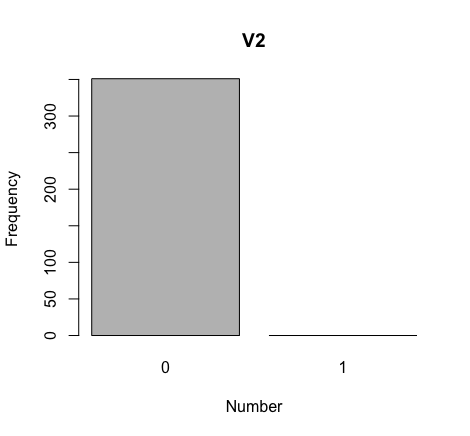
\includegraphics[width=6cm]{v2.png}
\pagebreak
\begin{lstlisting}[language=R]
v35 <- c(sum(mydata$V35 == "g"), sum(mydata$V35 == "b"))
barplot(
    v35,
    xlab = "Good Bad",
    ylab = "Frequency",
    main = "V35",
    names.arg = c("Good", "Bad")
)
\end{lstlisting}
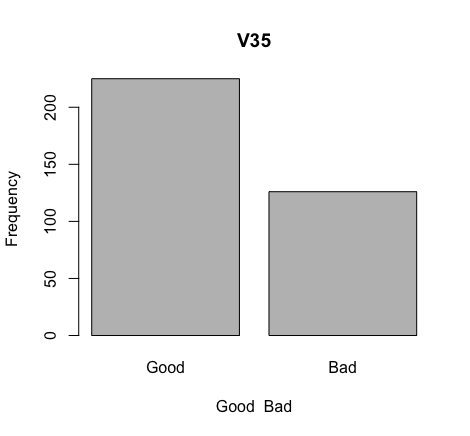
\includegraphics[width=6cm]{v35.png}
\pagebreak
\item[1.2.4]  Make a scatter plots of [$V22, V20$] and [$V1,V2$] variables and color the data points with the class variable [$V35$]. Discuss the plots, i.e., do you observe any relationships between variables?
\begin{lstlisting}[language=R]
chageToColor <- function (x) {
    for (i in 1:nrow(mydata)) {
        if (x[i] == "g") {
            x[i] <- "blue"
        } else {
            x[i] <- "red"
        }
    }
    return (x)
}
v35Color <- chageToColor(mydata$V35)
plot(
    mydata$V22,
    mydata$V20,
    xlab = "V22",
    ylab = "V20",
    main = "V22 & V20",
    col = v35Color
)
plot(
    mydata$V1,
    mydata$V2,
    xlab = "V1",
    ylab = "V2",
    main = "V1 & V2",
    col = v35Color
)
\end{lstlisting}
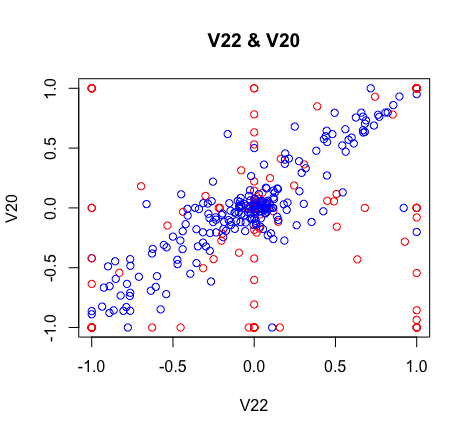
\includegraphics[width=8cm]{v22v20.png}
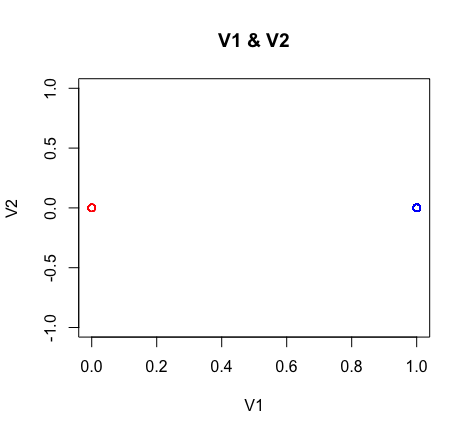
\includegraphics[width=8cm]{v1v2.png}
\end{enumerate}
\end{enumerate}

\pagebreak
%%%%%%%%%%%%%%%%%%%% PROBLEM 2  %%%%%%%%%%%%%%%%%%%% %%%%%%%%

\section*{Problem 2 [10 points]} 

The pseudo-code for $k$-means and a running example of $k$-means on a small data set are provided above. Answer the following questions:

\begin{enumerate}
  \item[2.1] Does $k$-means always converge? Given your answer, a bound on the iterate must be included. How is
its value determined?
\begin{verbatim}
$k$-means does not always converge, because for each time with the different initial 
points, the clusters might be different.
\end{verbatim}
  \item[2.2] What is the run-time of this algorithm?
\end{enumerate}

\pagebreak

%%%%%%%%%%%%%%%%%%%% PROBLEM 3  %%%%%%%%%%%%%%%%%%%% %%%%%%%%


\section*{Problem 3 [20 points]} 

 Implement Lloyd's algorithm for $k$-means (see algorithm $k$-means above)  in \textit{R} and call this program $C_k$. As you present your code explain your protocol for


\begin{enumerate}
  \item[3.1] initializing centroids
  \item[3.2] maintaining $k$ centroids
  \item[3.3]  deciding ties
  \item[3.4] stopping criteria
\end{enumerate}

\begin{lstlisting}[language=R]
dis <- function (p1, p2) {
    d <- 0
    for (i in 1:length(p1))
        d <- d + (p1[i] - p2[i]) * (p1[i] - p2[i])
    return (sqrt(d))
}

# stopping criteria
thresHold <- function(c1, c2, t, k, dataSet) {
    ans <- 0
    for (i in 1:k)
        ans <- ans + dis(c1[i, ], c2[i, ])
    ans <- ans / k
    return (ans < t)
}

k_means <- function (dataSet, dis, k, t) {
    # initial central point of each clusters
    len <- ncol(dataSet)
    cv <- matrix(nrow = k, ncol = len)
    cB <- matrix(nrow = k, ncol = nrow(dataSet) + 5)
    c_copy <- cv
    initialC <- sample(1:nrow(dataSet), k, replace = F)
    for (i in 1:k) {
        for (j in 1:len)
            cv[i, j] = dataSet[initialC[i], j]
        cB[i, 1] <- 2
    }
    
    # maintaining k centroids
    i <- 0
    while (i >= 0) {
        c_copy <- cv
        
        cB <- matrix(nrow = k, ncol = nrow(dataSet) + 5)
        for (j in 1:k)
            cB[j, 1] <- 2
        
        lo <- 0
        for (j in 1:nrow(dataSet)) {
            lo <- lo + 1
            minDis <- 0xfffffff
            n <- -1
            
            for (kk in 1:k) {
                p1 <- as.double(dataSet[j, ])
                p2 <- cv[kk, ]
                if (dis(p1, p2) < minDis) { # deciding ties
                    n <- kk
                    minDis <- dis(p1, p2)
                }
            }
            cB[n, cB[n, 1]] <- lo
            cB[n, 1] <- cB[n, 1] + 1
        }
        
        for (j in 1:k) {
            co <- c()
            for (kk in 1:len) {
                sum <- 0
                num <- 0
                l <- 2
                while (!is.na(cB[j, l])) {
                    xLoc <- cB[j, l]
                    yLoc <- kk
                    val <- as.double(dataSet[xLoc, yLoc])
                    sum <- sum + val
                    num <- num + 1
                    l <- l + 1
                }
                co <- c(co, sum / num)
            }
            cv[j,] <- co
        }
        
        # stopping criteria
        if (i > 0 && thresHold(c_copy, cv, t, k, dataSet))
            break
        i <- i + 1
    }
    
    return (list(v = cv, B = cB))
}

# test case
bigData <- data.frame(mydata[, 1:34])
k_means (bigData, dis, 5, 10)
tinyData <-
    matrix(c(2, 1, 22, 42, 15, 5, 5, 55, 12, 16),
           nrow = 5,
           ncol = 2)
tinyData <- data.frame(tinyData)
k_means (tinyData, dis, 2, 10)
\end{lstlisting} 

\pagebreak

%%%%%%%%%%%%%%%%%%%% PROBLEM 4 %%%%%%%%%%%%%%%%%%%% %%%%%%%%

 
\section*{Problem 4 [40 points]}
 
 In this question, you are asked to run  your program, $C_k$, against   \href{https://archive.ics.uci.edu/ml/datasets/ionosphere}{
Ionosphere Data Set}. Upon stopping, you will calculate the quality of the centroids and of the partition.  For each centroid $c_i$, form two counts:
  \begin{eqnarray*}
  g_i &\gets& \sum_{\delta \in c_i.B} [\delta.C =\text{\quotes{g}}],\ \ \ \mbox{\rm good}\\
  b_i &\gets& \sum_{\delta \in c_i.B} [\delta.C = =\text{\quotes{b}}], \ \ \ \mbox{\rm bad}
  \end{eqnarray*}
  where $[x = y]$ returns 1 if True, 0 otherwise.  For example, $[2 = 3] + [0 = 0] + [34 = 34] = 2$
  
  The centroid $c_i$ is classified as good if $g_i > b_i$ and bad otherwise.  We can now calculate a simple error rate.    Assume $c_i$ is good.  Then the error is:
 \begin{eqnarray*}
 error(c_i) &=& \frac{b_i}{b_i + g_i}
 \end{eqnarray*}
 We can find the total error rate easily:
 \begin{eqnarray*}
 Error(\{c_1, c_2, \ldots, c_k\}) &=& \sum_{i=1}^k error(c_i)
 \end{eqnarray*}

Report the total error rates for $k = 2,\ldots 5$ for 20 runs each, presenting the results that are easily understandable.  Plots are generally a good way to convey complex ideas quickly, i.e., box plot.  Discuss  your results.

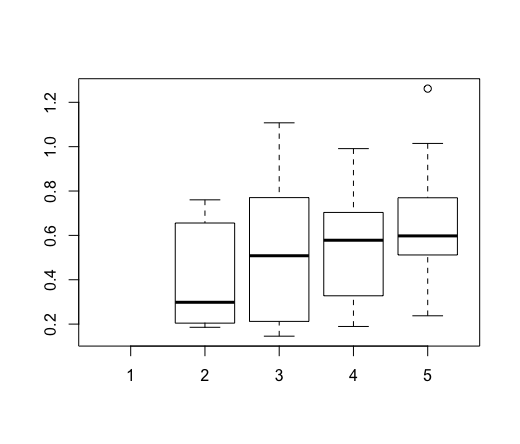
\includegraphics[width=10cm]{4.png}
\begin{verbatim}
For more clusters, there will be larger error rate!
\end{verbatim}
\pagebreak

%%%%%%%%%%%%%%%%%%%% PROBLEM 5  %%%%%%%%%%%%%%%%%%%% %%%%%%%%

 
 \section*{Problem 5 [10 points]} In this question, you are asked to make use of  the \href{https://stat.ethz.ch/R-manual/R-devel/library/stats/html/kmeans.html}{ R package for $k$-means.} Elbow method is one of the techniques to decide the optimal cluster number.  Find the optimal cluster number for Ionosphere data set using elbow method (for  $2 \leq k \leq 15$). Provide a plot that shows the total SSE for each $k$. Discuss your results.

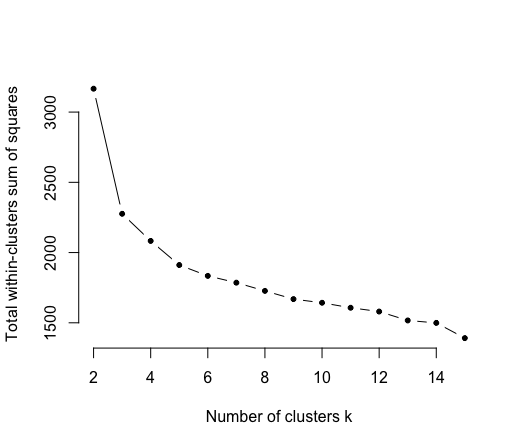
\includegraphics[width=10cm]{5.png}
\begin{verbatim}
I will consider 3 cluster will be better to choose, because through the graph, 
we can find a obviously turn at 3 clusters.
\end{verbatim}

\pagebreak

%%%%%%%%%%%%%%%%%%%% PROBLEM 6  %%%%%%%%%%%%%%%%%%%% %%%%%%%%
 
\section*{Problem 6 [10 points]}

Let $X \subset \mathbb{R}^n$  ($\mathbb{R}$ is the set of reals) for positive integer  $n>0$. Define a  distance $d: X \times X \rightarrow  \mathbb{R}_{\geq 0} $ as

\begin{equation*}
d(x,y) =  max\{|x_i - y_i|\}, \forall i\ 1\leq i \leq n
\end{equation*}

Prove/disprove $d$ is a metric?

\begin{verbatim}
According to three definition for metric:

(1) d(x, x) = max{|xi - xi|} = 0. And, if x!= y, then there exists some j which x!= y, 
    and consequently, |xi - yi| > 0. Therefore, d(x, y) = max{|xi - yi|} > 0 
(2) d(x, y) = max{|xi - yi|} = max{|yi - xi|} = d(y, x)
(3) If i = i,...,n. Then, 
    |(xi - zi)| = |(xi - yi) + (yi - zj)| <= |xi - yi| + |yi - zi|, by the Triangle Inequality 
    Use  max value over i = 1, ..., n of eqution:
    d(x, z) = max{|xi - ji|} <= max{|xi - ji| + |yi - zi|} <= max{|xi - yi|} + max{|yi - zi|} = d(x, y) + d(y, z), 
    Therefore,  d(x, z) <= d(x, y) + d(y, z)
    
Therefore, d is a metric.

\end{verbatim}

\pagebreak

%%%%%%%%%%%%%%%%%%%% Extra credit %%%%%%%%%%%%%%%%%%%% %%%%%%%%

\section*{Extra credit [30 points]}

This part is optional. 

\begin{enumerate}

\item[1] The $k$-means algorithm provided above stops when centroids become stable (Line  34). In theory, $k$-means converges once SSE is minimized
\begin{eqnarray*}
SSE = \sum_{j}^k \ \ \smashoperator{ \sum_{x \in c_j.B}} ||\mathbf{x} - c_j.v||^2_2 \label{costfunt}
\end{eqnarray*} 
 
In this question, you are asked to use SSE as stopping criterion. Run $k$-means over  \href{https://archive.ics.uci.edu/ml/datasets/breast+cancer+wisconsin+(original)}{ Breast Cancer Wisconsin Data Set} and report the total SSE  in a plot for $k = 2,\ldots ,5$ for 20 runs each. Discuss your results. [15 points].

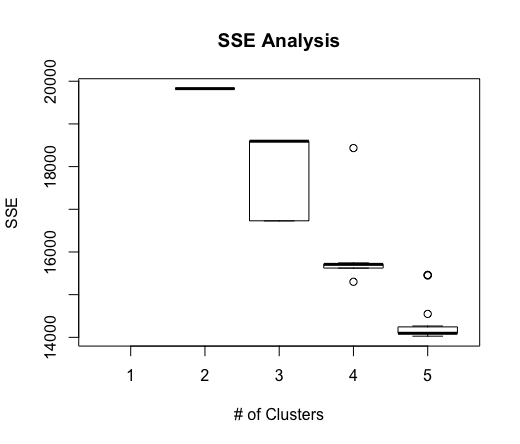
\includegraphics[width=10cm]{E1.png}
\begin{verbatim}
I will consider 3 cluster will be better to choose, because through the graph, 
we can find a obviously turn at 3 clusters.
\end{verbatim}

\item[2] Traditional $k$-means initialization is based on choosing values from a uniform distribution. In this question, you are asked to improve $k$-means through initialization.  \href{http://ilpubs.stanford.edu:8090/778/1/2006-13.pdf}{$k$-means ++} is an extended $k$-means clustering algorithm and induces non-uniform  distributions over  the data  that serve as  the initial centroids. Read the paper and discuss the idea in a paragraph.  Implement this idea to improve your $k$-means program. [15 points]
\end{enumerate}

\pagebreak

%%%%%%%%%%%%%%%%%%%%%%%%%%%%%%%%%%%%%%%%%%%%%%%%%%%%%%%%%%%%%%

\pagebreak
\section*{What to Turn-in}
 Submit a .zip file that includes the files below. Name the .zip  file as \quotes{usename-section number}, i.e., hakurban-B365.





\begin{itemize}
\item The *tex and *pdf of the written answers to this document.
\item *\texttt{R}files for:
\begin{itemize}
\item  implementation of $k$-means  [Problem 4] 
\item \texttt{R}  package  usage [Problem 5]
\item  extra  credit questions--optional
\end{itemize}
\item A README file that explains how to run your code and other files in the folder
\end{itemize}


 



\end{document}


